\section{Design of \name}
\begin{figure*}[htbp]
    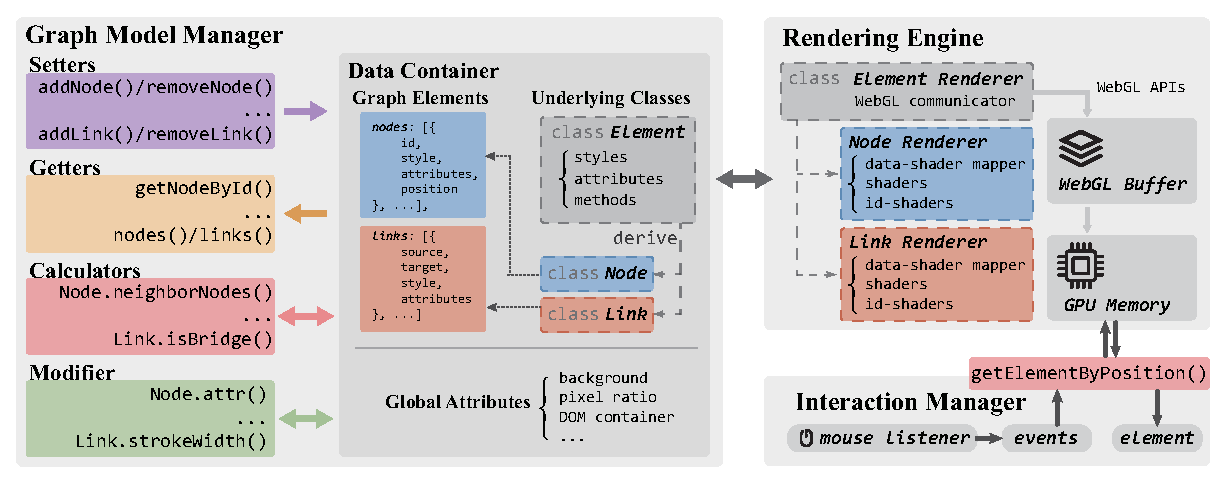
\includegraphics[width=\linewidth]{fig/architecture.eps}
    \caption{
        \name designs: \name consists of three parts: core engine, plugins, and library interface.
    }
    \label{fig:design}
\end{figure*}

% \begin{figure}[htbp]
%     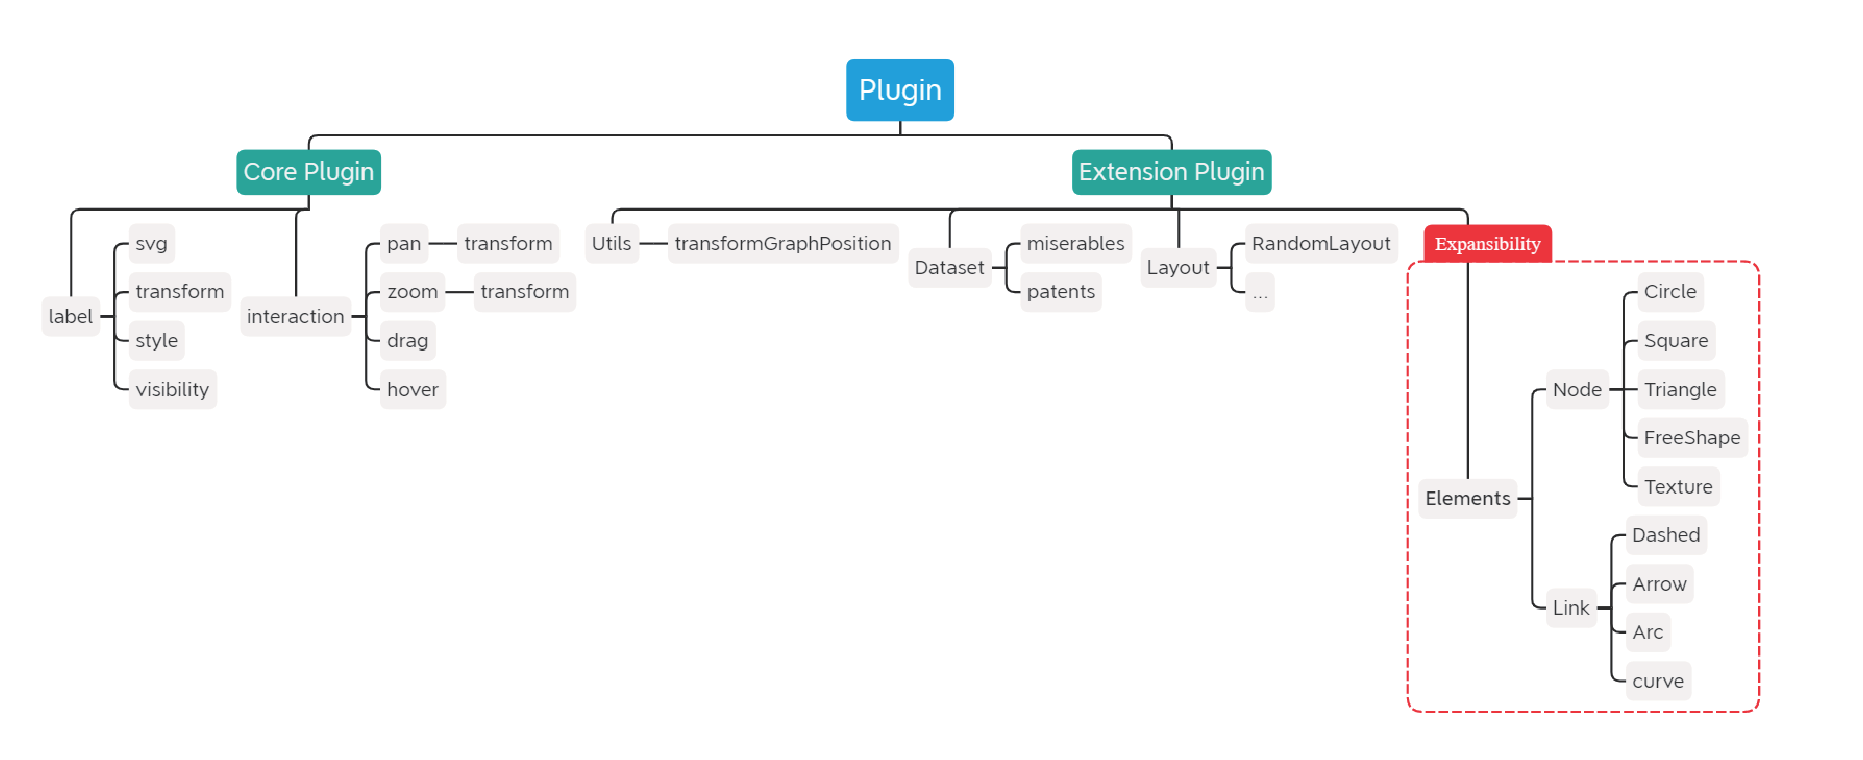
\includegraphics[width=\linewidth]{fig/xmind-02.eps}
%     \caption{
%         \name designs: \name consists of three parts: core engine, plugins, and library interface.
%     }
%     \label{fig:design}
% \end{figure}
% \begin{figure}[htbp]
%     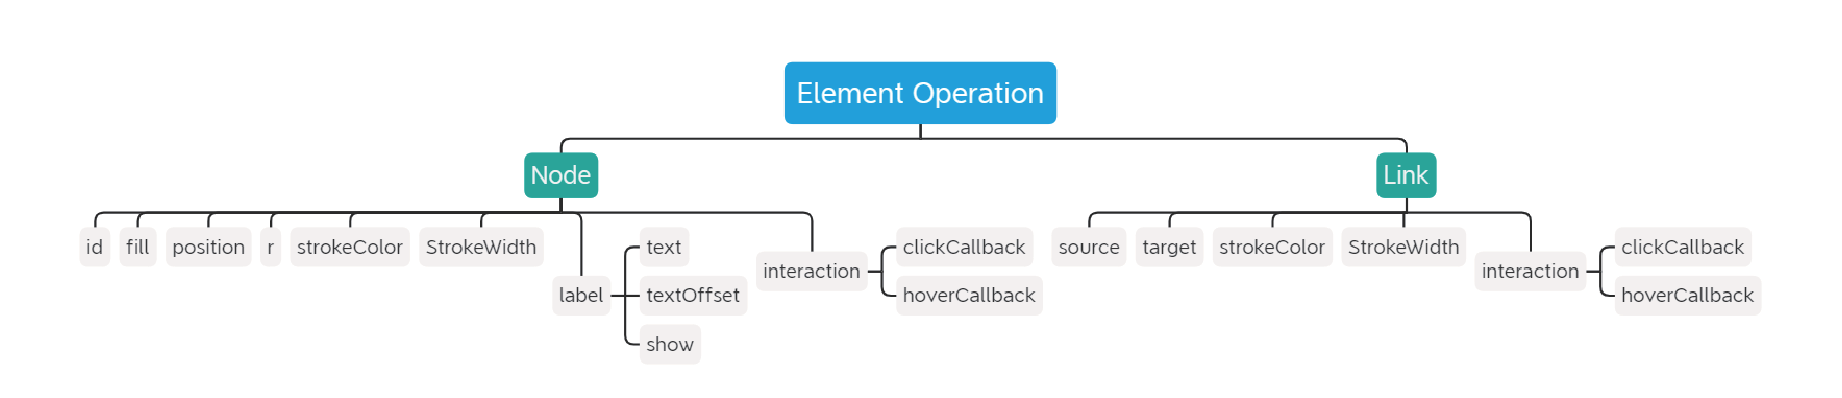
\includegraphics[width=\linewidth]{fig/xmind-03.eps}
%     \caption{
%         \name designs: \name consists of three parts: core engine, plugins, and library interface.
%     }
%     \label{fig:design}
% \end{figure}
% \begin{figure}[htbp]
%     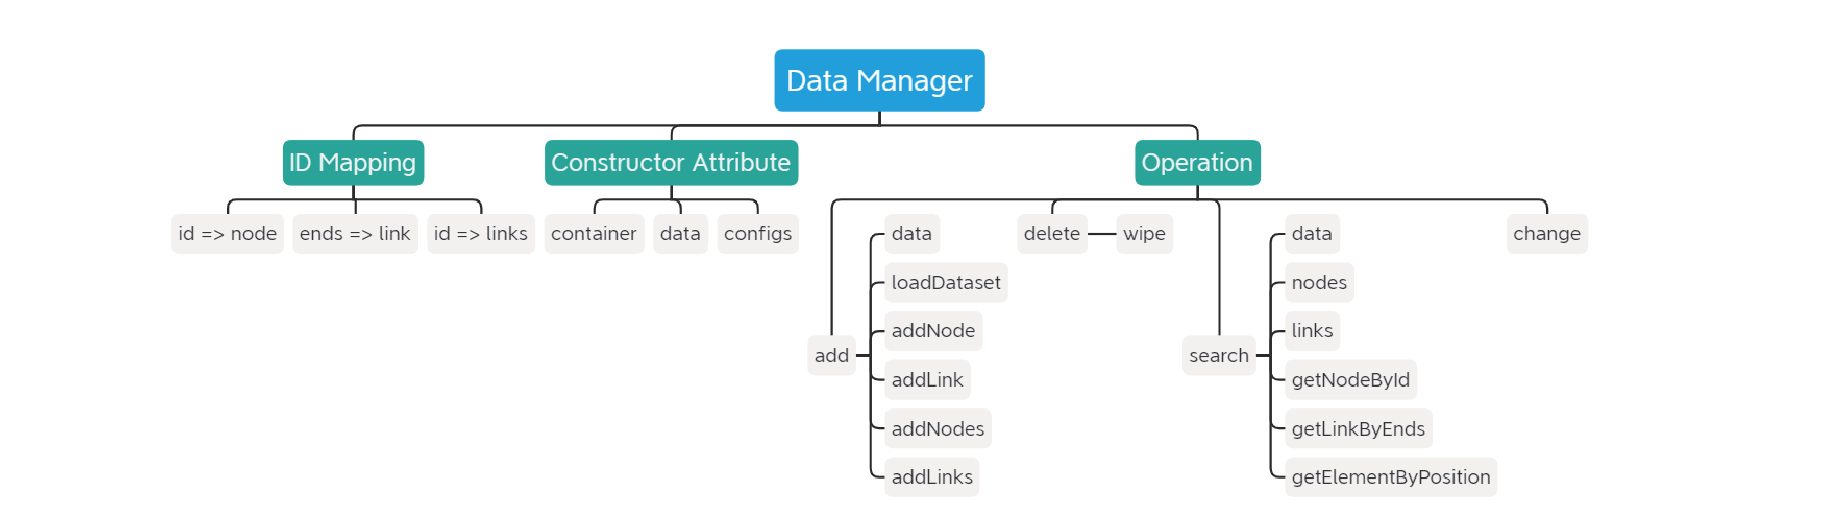
\includegraphics[width=\linewidth]{fig/xmind-04.eps}
%     \caption{
%         \name designs: \name consists of three parts: core engine, plugins, and library interface.
%     }
%     \label{fig:design}
% \end{figure}

\subsection {Design Requirements of \name}

\deleted[id=pan]{为了探索\name的设计空间,我们采访了3个图可视化相关的专家,调研了一系列图可视化的工具,包括 Gephi, Cytoscape.js, Sigma.js, GraphViZ,总结了如下高性能节点链接图可视化的设计需求:}

\added[id=pan] {To explore the design space of \name, we interviewed three graph visualization experts, investigated six graph visualization tools including Gephi~\cite{DBLP:conf/icwsm/BastianHJ09}, Pajek~\cite{DBLP:reference/snam/BatageljM14}, SNAP~\cite{leskovec2016snap}, Sigma.js~\cite{DBLP:journals/jossw/Coene18}, GraphViZ~\cite{Ellson03graphvizand}, and Cytoscape.js~\cite{DBLP:journals/bioinformatics/FranzLHDSB16}. We summarized the following design requirements for high-performance node-link diagram visualization: }

\begin{enumerate}
\renewcommand{\labelenumi}{\textbf{R\theenumi}}
\item \deleted[id=pan]{\textbf{需要有抽象的图模型来帮助控制图可视化}: 为了简化开发者对于可视化的操作,\name需要一个抽象图模型来控制图可视化而非直接控制图可视化的元素。该模型需要支持图的以下几点特性:}
\begin{enumerate}[R\theenumi.1]
    \item \deleted[id=pan]{\textbf{链接关联节点}: 每条链接都会关联到两个节点是图结构最基本的特性,该特性使得绘制节点链接图可以不关心链接的位置,开发者可以专注于节点的位置修改,链接会相应联动。}
    \item \deleted[id=pan]{\textbf{邻节点和邻接边的可访问性}: 我们在调研过程中发现,很多可视化系统中支持了高亮某个节点的邻接边和邻节点的交互。所有专家都一致同意为图模型增加邻节点和邻接边可访问功能的重要性。}
    \item \deleted[id=pan]{\textbf{基本图论算法的支持}: 部分算法提供了一些图论的基本算法,比如计算某些度量(如节点度数,节点centrality,图直径等),或是获取两个节点之间的最短路。专家们都一致同意图论算法对于可视化的重要性,但他们部分同意实现图论算法的必要性,其中一个专家认为该功能不属于可视化渲染库所关心的需求。}
\end{enumerate}
\item \deleted[id=pan]{\textbf{需要对拥有大量可视化元素的节点链接图提供高刷新率}: 根据我们对三位图可视化专家的采访,他们认为【对超过10万元素的大规模图有30fps以上的渲染速度】才能认为其对大规模节点链接图提供了高性能渲染的能力。}
\item \deleted[id=pan]{\textbf{支持不同节点和链接的样式}: 开发者往往需要在节点链接图上编码不同信息,虽然在大部分大规模图可视化案例中,圆形的节点和直线边最受欢迎,但仍然有很多节点链接图支持了不同形状的节点和不同样式的边。因此,为节点和链接赋予不同的形状和样式,能使得开发者有更多可以编码信息的空间。}
\item \deleted[id=pan]{\textbf{需要提供多种布局功能和自定义布局插件}:节点链接图对于布局的依赖程度不言而喻。\name 需要提供一些基础的节点链接图布局。因为布局算法的多样性,\name 还需能使开发者按照既定接口接入自定义布局。}
\item \deleted[id=pan]{\textbf{需要提供自定义标签渲染}:虽然在渲染大规模节点链接图时,为可视化元素赋予标签会导致visual clutter的问题,但开发者仍有可能采取某些策略来绘制标签,比如在屏幕内元素数量较少时自适应地绘制标签。所以,\name有必要提供标签绘制的接口。}
\item \deleted[id=pan]{\textbf{需要提供基础交互模型}:虽然对于节点链接图的交互多种多样,但根据我们的调研和专家访谈,我们发现它们基本上都可以被分解为对节点、链接以及画布的交互监听。我们认为\name需要能够对节点进行拖拽、点击、鼠标悬浮的监听,对链接需要有点击和鼠标悬浮的监听,以及对画布需要能够有平移、缩放、点击的交互监听。我们还需要实现对节点链接图的可视化元素的选择功能,比如lasso。}
\end{enumerate}

\subsection{Design Details of \name}
\newcommand{\RenEng}{\textit{Rendering Engine}}
\newcommand{\GraModMan}{\textit{Graph Model Manager}}
\newcommand{\IntMan}{\textit{Interaction Manager}}

\deleted[id=pan]{为了完成上述的需求,我们设计实现了 \name。\name 包含了三个主要部分:\GraModMan 、\RenEng 以及 \IntMan 。我们还将一些非核心的需求独立抽象为插件的形式方便开发者自定义调用,从而减少\name的核心代码。}

\subsubsection{\GraModMan}
为了能够有抽象的图模型来帮助图可视化,我们在\name中设计实现了\GraModMan,一个图模型的控制器(图1)。该控制器的主体是一个Data Container,其存储了节点数据和链接数据。每个节点拥有一个唯一标志符id,其对应的样式会被存储在style属性中,而位置坐标责备存储在position中,其余的属性则会被存储在attributes中;同样的,每个link都拥有一个source和一个target,代表它所关联的两个节点,其对应的样式和其余属性会被存储在style和attributes中。我们为节点和链接建立了对应的class:Node和Link来存储每一个数据实体。他们派生自Element类。

我们为data elements (nodes和links) 设计了 增、删、改、查和计算的功能。开发者可以通过data setter来增加和删除elements,通过 data getter 则能用于查询element, 通过 data modifier 修改数据的内容(如属性、样式等)。除此以外,我们还提供了部分常用的图计算的接口,因为该部分和可视化的关联并不紧密,我们只实现了部分功能,比如查询节点的邻节点等。

\subsubsection{\RenEng}
为了满足\textbf{R2},\RenEng 调用了GPU的高性能渲染来绘制可视化。
\subsubsection{\IntMan}

% % \name aims to help users rapidly and efficiently construct network visualization applications.
% % Specifically, \name consists of three parts: the core engine, plugins, and library interface (\autoref{fig:design}).
% % The core engine contains the data manager for maintaining nodes and links and the renderer for leveraging GPU processing power to render a large-scale network.
% % The plugins are employed to increase and expand more requirements and functions.
% % The library interface aims to help developers rapidly construct applications with friendly and concise APIs.


% % \subsection{Core Engine}
% % The core engine aims to render large-scale network based on WebGL and maintains the primary network information for rapidly editing operations.
% % It consists of the data manager and the renderer.

% % \subsubsection{Data Manager}
% % The data manager supports a series of interface corresponding network structure.
% % It is used to achieve nodes or links operations, including adding, deleting, searching, and editing.
% % Node-links and link-nodes mapping tables are also supported for accelerating search and locate.
% % At the same time, the data manager has a build-in network data set for developers to get started quickly.

% % \subsubsection{Renderer}
% % The renderer aims to render basic elements: nodes and links. It focuses on the efficiency of rendering massive data on the browser platform. As the highest performance graphics rendering API of browser platform, \name uses WebGL as the bottom rendering.
% % However, WebGL programming is still hard and complex.
% % The WebGL API is encapsulate
% % In order to reduce the program execution time as much as possible, the basic WebGL API is only encapsulated to meet the most basic data processing and rendering.
% % Specifically, the renderer uses three strategies to improve rendering efficiency.

% \begin{itemize}
% \item \textbf{Batch}: The renderer contains a batch drawing element instance. Considering that most of the elements of the network are the same, but the location information is different. The renderer creates an instance of an element and draws it in the batch process to reduce the consuming time of the rendering process.

% \item \textbf{Shader}: The renderer uses Shader function to control the shape render. Each node's shape usually needs to be defined as a circle, square, ellipse, and so on. However, the complex shape will cause a serious effect on rendering performance.
% \name exploits the powerful Shader function to define and render shape in GPU with batch processing.

% \item \textbf{Modify as needed}: The renderer supports manual rendering function for developers.
% The main attributes of elements, including positions, color, and texture, are stored into different buffers of GPU.
% When attributes of elements need to be Modified, the renderer can refresh corresponding buffers rather getting attributes from the data manager. And then, developers can refresh the network by supported function. The time consuming of getting attributes from the data manager can be omitted.

% \item \textbf{Element positioning}: The renderer has an elements positioning function for supporting elements search and interaction. For improving user interaction efficiency, the renderer uses the WebGL Texture to record the screen pixel position of each element.
% The time consuming of elements positioning has great improvement compared with index search and spatial index tree.
% The time complexity of the function is $O(1)$.

% \end{itemize}

% \subsection{Plugin module}
% The goal of the plugin modular is to enhance future expansions.
% For supporting more features and requirements, \name designs the plugin modular to employ new improvements or functions.
% At the same time, it can isolate the core modular from the rest.
% For now, the plugin module includes:
% \begin{itemize}
%     \item \textbf{Interaction: } It supports binding interaction events and callback functions of elements. Interaction events contain basis events of edges and nodes such as Hover, MouseDown, Click, etc.
%     \item \textbf{Layout: } It contains build-int layouts and allows users to use custom layouts.

% \end{itemize}

% \subsection{Library Interface}
% The library interface aims to support concise and efficient API for users to build large-scale network visual analysis applications quickly.
% Users do not need to touch the underlying WebGL rendering programming. Humanized and simple API can be called to config data and render network.
% Specifically, it includes three parts:
% \begin{itemize}
%     \item \textbf{Global: }It is used to define custom configs, such as the mount node, the default style of the canvas, and the default style of elements.
%     \item  \textbf{Element: }It includes the data adding of nodes of edges and the attributes changing of elements.
%     \item  \textbf{Plugin: }It aims to set up different plugins, such as layouts and interactions.
% \end{itemize}
